\documentclass[11pt]{article}
\usepackage[utf8]{inputenc}
\usepackage[a4paper,margin=1in]{geometry}
\usepackage{amsmath,amssymb}
\usepackage{hyperref}
\usepackage{enumitem}
\usepackage{titlesec}
\usepackage{xcolor}
\usepackage{fancyhdr}
\usepackage{tikz}
\usepackage{graphicx}
\usepackage{eso-pic}

\graphicspath{{../}}

\definecolor{kcpc-text}{RGB}{20,20,20}
\definecolor{kcpc-muted}{RGB}{90,90,90}
\definecolor{kcpc-red}{RGB}{176,0,0}

\pagestyle{fancy}
\fancyhf{}
\lhead{\textcolor{kcpc-text}{\small\bfseries Papers}}
\rhead{\textcolor{kcpc-muted}{\small Week 4}}
\cfoot{\textcolor{kcpc-muted}{\small KCPC}}
\renewcommand{\headrulewidth}{0.4pt}
\renewcommand{\headrule}{\hbox to\headwidth{\color{kcpc-red}\leaders\hrule height \headrulewidth\hfill}}
\renewcommand{\footrulewidth}{0pt}
\setlength{\headheight}{28pt}

\AddToShipoutPictureBG{%
    \begin{tikzpicture}[remember picture,overlay]
        \node[opacity=0.035, at=(current page.center)]
        {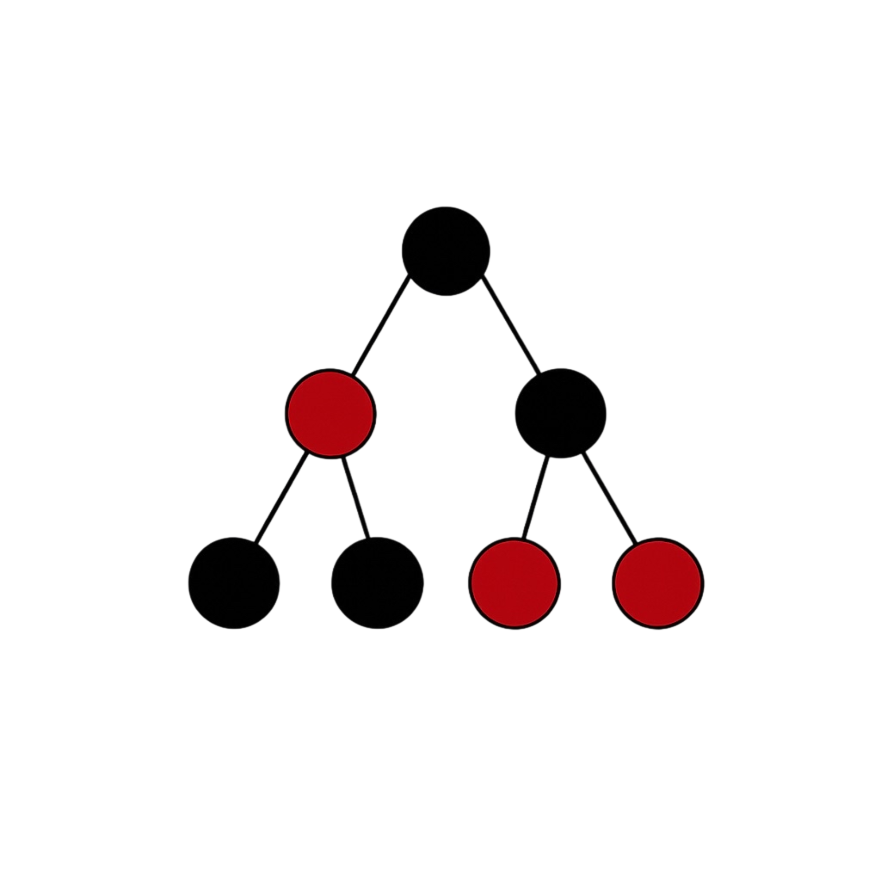
\includegraphics[width=0.38\paperwidth]{kcpc-logo.png}};
    \end{tikzpicture}%
}

\titleformat{\section}{\large\bfseries\color{kcpc-red}}{}{0pt}{}
\titleformat{\subsection}{\normalsize\bfseries}{\thesubsection}{1em}{}

\hypersetup{
    colorlinks=true,
    linkcolor=kcpc-red,
    urlcolor=kcpc-red
}

\title{KCPC Week 4 Papers\\Foundations of Graph Theory, Traversals, and Structural Algorithms}
\author{King's Competitive Programming Club\\
  \small Curated by Mehmet Kutay Bozkurt (\href{https://github.com/mkutay}{@mkutay})}
\date{}

\begin{document}

\maketitle
\thispagestyle{fancy}

\noindent
This annotated bibliography compiles the foundational research papers behind Workshop 4 (\textit{Introduction to Graphs}). Each entry provides a complete citation, a persistent link or archive location, and the exact sections and page numbers relevant to the workshop slides and problem sheet. For textbook introductions and competitive programming tutorials, see \emph{Week 4 Reading}.

\section*{I. Origins of Graph Theory and Degree Invariants}

\subsection*{[1] Euler, L. (1736 / published 1741)}
\textit{Solutio problematis ad geometriam situs pertinentis.}
Commentarii Academiae Scientiarum Imperialis Petropolitanae, 8, 128--140.
\url{https://scholarlycommons.pacific.edu/euler-works/53/}

\textbf{Where / why:}
Paragraphs 1--21 (pp.~128--140) formulate the Seven Bridges of K{\"o}nigsberg by stripping away metric geometry and retaining only discrete vertices (landmasses) and edges (bridges). Paragraphs 11--20 establish how vertex degrees govern walks and parity ($\sum_{v \in V} \deg(v) = 2|E|$). This paper is the historical origin of graph theory and underpins the degree-characterisation technique used in Slide Section 1 and Problem 2.2 (\emph{Cyclic Components}).

\section*{II. Breadth-First Search and Shortest Unweighted Paths}

\subsection*{[2] Moore, E. F. (1959)}
\textit{The shortest path through a maze.}
In \textit{Proceedings of an International Symposium on the Theory of Switching} (Harvard University, April 2--5, 1957), Part II, The Annals of the Computation Laboratory of Harvard University, Vol.~30, pp.~285--292. Harvard University Press.

\textbf{Where / why:}
Pages 285--288 introduce Breadth-First Search (Algorithms A and B) as a wavefront expansion across unweighted graphs and prove that labelling vertices in non-decreasing distance layers guarantees a minimum-edge path, reconstructed by tracing predecessor steps backward from the destination. Directly underpins Slide Section 3, Problem 1.2 (\emph{Message Route}), and Problem 3.1 (\emph{Rudolf and Subway}).

\subsection*{[3] Lee, C. Y. (1961)}
\textit{An algorithm for path connections and its applications.}
IRE Transactions on Electronic Computers, EC-10(3), 346--365.
\url{https://doi.org/10.1109/TEC.1961.5219222}

\textbf{Where / why:}
Sections I--II (pp.~346--351) independent of Moore formalise wave-propagation breadth-first search and parent back-tracing in discrete routing networks, proving optimality of the reconstructed path.

\section*{III. Depth-First Search, Linear-Time Representations, and Edge Classification}

\subsection*{[4] Tarjan, R. E. (1972)}
\textit{Depth-first search and linear graph algorithms.}
SIAM Journal on Computing, 1(2), 146--160.
\url{https://doi.org/10.1137/0201010}

\textbf{Where / why:}
Section 2 (pp.~146--150) formalises recursive Depth-First Search on adjacency lists, defines entry/exit vertex numbering, proves the $O(|V| + |E|)$ time bound, and establishes the structure of the DFS palm tree---showing that in an undirected graph every non-tree edge is a back-edge (frond) between an ancestor and a descendant, while directed graphs also admit cross and forward arcs. Directly underpins Slide Sections 2 and 4, Problem 1.1 (\emph{Building Roads}), and Problem 1.3 (\emph{Round Trip}).

\subsection*{[5] Hopcroft, J., \& Tarjan, R. (1973)}
\textit{Algorithm 447: Efficient algorithms for graph manipulation.}
Communications of the ACM, 16(6), 372--378.
\url{https://doi.org/10.1145/362248.362272}

\textbf{Where / why:}
Pages 372--375 detail concrete linear-space adjacency-list storage and $O(V + E)$ DFS routines for decomposing graphs into connected and biconnected components and extracting fundamental cycles.

\section*{IV. Bipartite Graphs and 2-Colouring}

\subsection*{[6] K\H{o}nig, D. (1916)}
\textit{{\"U}ber Graphen und ihre Anwendung auf Determinantentheorie und Mengenlehre.}
Mathematische Annalen, 77(4), 453--465.
\url{https://doi.org/10.1007/BF01456961}

\textbf{Where / why:}
Section 1, Theorem 2 (pp.~453--456) proves the foundational bipartite characterisation theorem: a graph is 2-colourable (bipartite) if and only if it contains no cycle of odd length. Directly underpins Slide Pattern 3, Problem 1.4 (\emph{Building Teams}), and the auxiliary bipartite graph construction in Problem 3.1 (\emph{Rudolf and Subway}).

\section*{V. Topological Sorting, DAGs, and Tree Diameter}

\subsection*{[7] Kahn, A. B. (1962)}
\textit{Topological sorting of large networks.}
Communications of the ACM, 5(11), 558--562.
\url{https://doi.org/10.1145/368996.369025}

\textbf{Where / why:}
Pages 558--560 present Kahn's in-degree algorithm: repeatedly extracting vertices of in-degree $0$ and decrementing the in-degrees of their successors produces a topological ordering of any Directed Acyclic Graph (DAG) in linear time, and detects directed cycles when non-extracted vertices remain. Directly underpins Slide Pattern 5, Problem 2.3 (\emph{DAG Number of Routes}), Problem 2.4 (\emph{Longest Path}), and cycle/tree separation in functional graphs.

\subsection*{[8] Handler, G. Y. (1973)}
\textit{Minimax location of a facility in an undirected tree graph.}
Transportation Science, 7(3), 287--293.
\url{https://doi.org/10.1287/trsc.7.3.287}

\textbf{Where / why:}
Section 1 (pp.~287--290) proves the two-sweep tree diameter theorem (originally observed for unweighted trees by Dijkstra around 1960): starting from an arbitrary vertex $r$ in a tree, any vertex $u$ at maximum distance from $r$ is an endpoint of a longest path, so a second traversal from $u$ finds the tree diameter in $O(V)$ time without dynamic programming. Directly underpins Slide Pattern 4 and Problem 2.5 (\emph{Tree Diameter}).

\end{document}
